\subsection{Work Breakdown Structure}
La Work BreakDown Structure, d'ora in poi WBS, rappresenta l'insieme delle attivit\`{a} necessarie a svolgere un compito ben preciso o un processo. Le singole attivit\`{a} prendono il nome di Work Package, WP, e definiscono dettagliatamente le azioni da svolgere per
ciascuna di esse.\\
La WBS \`{e} costituita da una struttura ad albero di WP che, a partire dell'obiettivo finale del progetto, specifica per suddivisioni successive i singoli sotto-obiettivi, fino all'unit\`{a} minima di attivit\`{a}.\\
Tale scomposizione in tanti compiti di dimensioni limitate facilita la gestione, il controllo e l'assegnazione delle singole attivit\`{a}, consentendo una migliore suddivisione del lavoro.\\
Grazie alla WBS il project manager pu\`{o}, in maniera semplificata, organizzare tutte le attivit\`{a} che compongono il progetto, cos\`{i} come i WP, ed avere sempre a disposizione un utile strumento che definisce tutti i passi necessari alla buona realizzazione del progetto.\\
La WBS, inoltre, risulta essere la base per tutte le altre attivit\`{a} di pianificazione richieste per la realizzazione di un progetto di successo.

\begin{figure}[H]
\centering % per centrare l'immagine (opzionale)
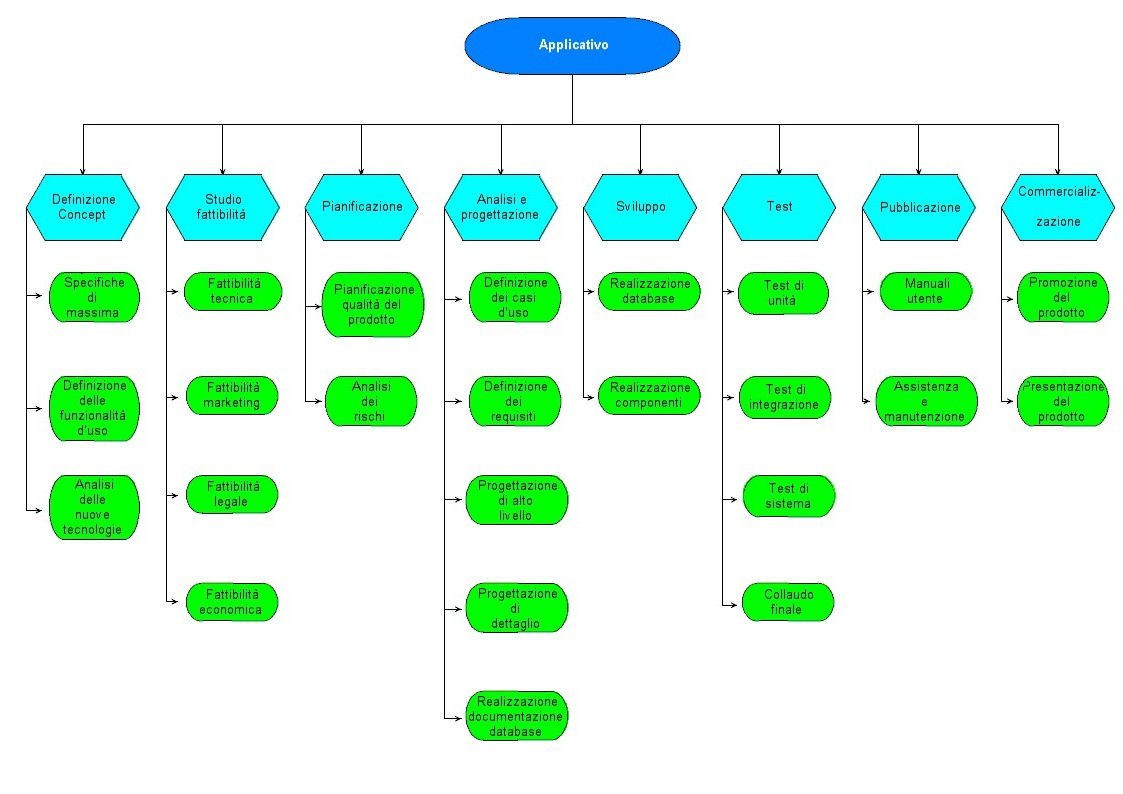
\includegraphics[scale=0.5]{img/Progetto.jpg}
\caption{Diagramma WBS}
\label{fig:Diagramma WBS}
\end{figure}

\subsubsection{WBS-Primo Livello}
\paragraph{Definizione Concept (1.1)}
\`{e} la prima fase del progetto, dove si raccolgono le idee per portare alla nascita e alla definizione del progetto.\\
A partire da questo momento in poi si penser\`{a} alla forma che assumer\`{a} il prodotto finale, alla  definizione delle caratteristiche pi\`{u} importanti (target del prodotto, come si intende erogare il servizio) e alla definizione delle funzionalit\`{a} principali che il prodotto finale deve avere.

\paragraph{Studio Fattibilit\`{a} (1.2)}
\`{e} la fase successiva a quella di Definizione Concept, ha lo scopo di capire se quello che si vuole realizzare \`{e} innanzitutto fattibile e possa portare ad avere dei guadagni concreti.\\
Dunque il concept viene valutato sotto tutti i punti di vista e di interesse per l'organizzazione, al fine di avere un insieme di conclusioni e indicazioni sulle possibilit\`{a} di buona riuscita del lavoro.

\paragraph{Pianificazione (1.3)}
In questa fase si vogliono studiare i processi che il team vuole adottare, quindi una pianificazione delle attivit\`{a} inerenti il ciclo di vita del prodotto avvalendosi di strumenti come diagrammi di Gantt, WBS, OBS e altri strumenti consultabili alla sezione Pianificazione. In questa fase si vogliono definire anche gli obiettivi e le strategie al fine di stabilire a priori ci\`{o} che il team dovr\`{a} controllare e soprattutto misurare.

\paragraph{Analisi e Progettazione (1.4)}
A questo punto gli obiettivi del progetto sono chiari, bisogna dunque formalizzarli e chiarirli in maniera non ambigua.\\
Vengono illustrate dettagliatamente le funzionalit\`{a}, i servizi e le prestazioni che dovranno essere offerte dal prodotto finito.\\
Infine viene progettato come il prodotto soddisfer\`{a} i requisiti definiti in precedenza, definendone la struttura ed architettura da assumere e rispettare.

\paragraph{Sviluppo (1.5)}
In questa fase si passa alla creazione vera e propria del prodotto software mediante la codifica di quanto definito durante la progettazione.\\
Affinché questo risulti possibile \`{e} essenziale che ogni membro si attenga strettamente a quanto descritto nei documenti che gli vengono forniti.\\
Non deve, assolutamente, inserire della creativit\`{a} personale, in quanto il suo compito consiste nella traduzione in codice di quanto deciso precedentemente.\\
Il codice prodotto dovr\`{a} essere costantemente verificato, per avere la sicurezza e la certezza che rispetti i requisiti di qualit\`{a} definiti nella fase di pianificazione, accompagnato dall'appropriata manualistica.

\paragraph{Test (1.6)}
Arrivati a questo punto vengono dunque effettuati i test delle componenti prodotte, verificando come si relazionano tra di loro, a partire dalle componenti di base del prodotto per arrivare a testare, alla fine, il sistema completo.\\
Inoltre viene verificato che quanto \`{e} stato prodotto sia conforme agli obiettivi e ai requisiti che si erano definiti in precedenza.

\paragraph{Post vendita (1.7)}
Una volta che il software prodotto \`{e} terminato e rispetta gli obiettivi ed i requisiti, viene avviato il piano per il rilascio.\\
In questa fase \`{e} prevista la realizzazione di documentazione a supporto dell'utente finale ed eventuali attivit\`{a} di manutenzione o comunque di supporto all'utente finale.\\

\paragraph{Commercializzazione (1.8)}
Questa fase \`{e} stata pianificata al fine di definire come la societ\`{a} intende promuovere il proprio prodotto, ricercare eventuali partnership.

\subsubsection {WBS-Secondo livello}
Per la descrizione dei Work Package di secondo livello verr\`{a} utilizzato il seguente schema in quanto,
, rappresentano tutti insiemi di attivit\`{a} elementari da realizzare:
\begin{description}
\item[Descrizione:] descrizione generica su ci\`{o} che il WP si propone di fare.
\item[Responsabile:] persona che ha la responsabilit\`{a} delle attivit\`{a} da svolgere nel WP e dell'output finale.
\item[Input:] Ci\`{o} di cui necessita in ingresso il WP per iniziare a svolgere le sue attivit\`{a}. Solitamente questi input vengono forniti in uscita da altri WP e possono essere prototipi, documenti o risorse.
\item[Output:] ci\`{o} che il WP deve produrre in uscita. I tipi di uscita possono essere diversi, a seconda delle attivit\`{a} svolte.
\item[Attivit\`{a}:] lista delle attivit\`{a} elementari necessarie al completamento del WP. Per poter essere considerato concluso un WP devono essere concluse tutte le sue attivit\`{a}.
\item[Costo:] costo in euro riassuntivo di tutte le spese necessarie al compimento del WP. Andranno considerate le spese relative al consumo di tutte le risorse utilizzate.
\item[Tempi di realizzazione:] tempo necessario stimato per la buona riuscita e per il completamento del WP, espresso in giorni lavorativi.
\end{description}

\paragraph{Specifiche di massima (1.1.1)}
\begin{description}
\item[Descrizione:] Definizione delle prime specifiche del prodotto per individuare i requisiti ad alto livello necessari a sviluppare l'abstract.
\item[Responsabile:]
\item[Input:] idee, critiche e specifiche provenienti da un brainstorming di gruppo.
\item[Output:] documento formale che descrive una prima versione della specifica del prodotto, nella quale si definisce dettagliatamente l'idea che si vuole realizzare.
\item[Attività:]\mbox{}\\[-1.5\baselineskip]
	\begin{itemize}
	\item ricerca nel web di eventuali competitors per ricavare da progetti gi\`{a} esistenti quali funzionalit\`{a} \`{e} bene riproporre, quali no e quali sono quelle innovative che bisogna sviluppare;
	\item brainstorming tra le risorse umane assegnate al WP per identificare caratteristiche da implementare nel prodotto;
	\item prima stesura documento;
	\item verifica documento ed eventuali correzioni;
	\item formalizzazione documento;
	\item approvazione;
	\end{itemize}
\item[Costo:] 270 \euro{}

\paragraph{Definizione delle funzionalit\`{a} d'uso (1.1.2)}
\begin{description}
\item[Descrizione:] definizione dettagliata delle pi\`{u} importanti funzionalit\`{a} che si vuole siano presenti all'interno del software.
\item[Responsabile:]
\item[Input:] documento di specifiche di massima prodotto dal WP.
\item[Output:] documento che descrive nel dettaglio le funzionalità base che si è deciso di sviluppare.
\item[Attività:]\mbox{}\\[-1.5\baselineskip]
	\begin{itemize}
	\item studio del documento prodotto dal WP;
	\item analisi tecnica di sistemi simili gi\`{a} esistenti;
	\item prima stesura del documento;
	\item verifica del documento ed eventuali correzioni;
	\item formalizzazione del documento;
	\item approvazione.
	\end{itemize}
\item[Costo:] 385 \euro{}
\item[Tempi di realizzazione:] 4 giorni lavorativi.
\end{description}

\paragraph{Analisi delle nuove tecnologie (1.1.3)}
\begin{description}
\item[Descrizione:] ricerca mirata di eventuali innovazioni tecnologie presenti nel mercato che possano risultare utili allo sviluppo del software.
\item[Responsabile:]
\item[Input:] documento di specifiche di funzionalit\`{a} prodotto dal WP.
\item[Output:] documento che descrive nel dettaglio eventuali nuove tecnologie interessanti che potrebbero essere inserite nel progetto. Per ciascuna di queste viene riportata una stima di tempo che si presuppone sia necessario ai programmatori per arrivare ad averne una buona padronanza.
\item[Attività:]\mbox{}\\[-1.5\baselineskip]
	\begin{itemize}
	\item studio del documento prodotto dal WP;
	\item analisi mirata di eventuali nuove tecnologie e stima delle ore per l'apprendimento;
	\item prima stesura documento;
	\item verifica documento ed eventuali correzioni;
	\item formalizzazione documento;
	\item approvazione.
	\end{itemize}
\item[Costo:] 279 \euro{}
\item[Tempi di realizzazione:] 3 giorni lavorativi.
\end{description}

\paragraph{Fattibilit\`{a} tecnica (1.2.1)}
\begin{description}
\item[Descrizione:] fase di valutazione del prodotto che si vuole realizzare dal punto di vista tecnico-tecnologico.
\item[Responsabile:] 
\item[Input:] tutti i documenti prodotti dal secondo livello del WP.
\item[Output:] documento che descrive nel dettaglio, in modo non ambiguo, la fattibilità tecnica per il prodotto che si vuole realizzare indicando le tecnologie e gli strumenti necessari per farlo.
\item[Attività:]\mbox{}\\[-1.5\baselineskip]
	\begin{itemize}
	\item studio dei documenti prodotti dai WP;
	\item incontro fra responsabili i tecnici;
	\item valutazione dei sistemi e degli standard in uso;
	\item valutazione delle tecnologie;
	\item prima stesura documento riassuntivo;
	\item verifica documento ed eventuali correzioni;
	\item formalizzazione documento;
	\item approvazione;
	\end{itemize}
\item[Costo:] 335 \euro{}
\item[Tempi di realizzazione:] 3 giorni lavorativi.
\end{description}

\paragraph{Fattibilit\`{a} marketing (1.2.2)}
\begin{description}
\item[Descrizione:] fase di analisi del mercato per studiare la concorrenza dovuta ad idee similari. Seguono quindi una stima ed una analisi della redditivit\`{a} del prodotto e alle indicazioni preliminari su come pubblicizzarlo e rilasciarlo al fine di ottenere maggiori introiti dalla vendita.
\item[Responsabile:] 
\item[Input:] ricerche di mercato e dati riguardanti eventuali competitor.
\item[Output:] documento formale che indica la fattibilità dal punto di vista del marketing. Nel caso di una buona riuscita sono riportate anche le azioni da seguire per il rilascio del prodotto.
\item[Attività:]\mbox{}\\[-1.5\baselineskip]
	\begin{itemize}
	\item analisi di mercato;
	\item interviste, sondaggi e dialoghi con possibili clienti;
	\item individuazione di eventuali strategie;
	\item prima stesura documento riassuntivo;
	\item verifica documento ed eventuali correzioni;
	\item formalizzazione documento;
	\item approvazione;
	\end{itemize}

\item[Costo:] 319 \euro{}
\item[Tempi di realizzazione:] 3 giorni lavorativi.
\end{description}
\paragraph{Fattibilit\`{a} legale (1.2.3)}
\begin{description}
\item[Descrizione:] fase di analisi del prodotto software sotto l'aspetto legale. Si studiano e si definiscono le strategie eventuali da adottare in difesa del progetto. Si verifica inoltre la possibilit\`{a} di brevettare il prodotto e di registrare un marchio. Infine si verifica che lo sviluppo non porti alla violazione di alcuna legge o normativa in vigore.
\item[Responsabile:]
\item[Input:] conoscenza di eventuali prodotti simili nel mercato e normative/vincoli legali.
\item[Output:] documento formale che indica la fattibilità dal punto di vista legale. Se viene prevista una buona riuscita allora sono riportate anche le azioni da seguire per il corretto rilascio del prodotto.
\item[Attività:]\mbox{}\\[-1.5\baselineskip]
	\begin{itemize}
	\item definizione di un marchio;
	\item consulenza esterna legale;
	\item prima stesura documento riassuntivo;
	\item verifica documento ed eventuali correzioni;
	\item formalizzazione documento;
	\item approvazione;
	\end{itemize}

\item[Costo:] 315 \euro{}
\item[Tempi di realizzazione:] 3 giorni lavorativi.
\end{description}
\paragraph{Fattibilit\`{a} Economica (1.2.4)}
\begin{description}
\item[Descrizione:] fase di analisi del prodotto software sotto l'aspetto economico. Si studia e si valutano i benefici economici che tale progetto potrebbe portare. Vengono stimati inoltre i costi che l'organizzazione dovrebbe sostenere, diretti ed indiretti. Inoltre viene studiata la possibilit\`{a} di ottenere dei finanziamenti esterni 
\item[Responsabile:] 
\item[Input:] conoscenza dei costi diretti ed indiretti delle varie risorse.
\item[Output:] documento formale che indica la fattibilità dal punto di vista economico. All'interno di questo verrà illustrata la previsione economica del prodotto, illustrando i possibili guadagni ed indicando l'eventuale punto di pareggio.
\item[Attività:]\mbox{}\\[-1.5\baselineskip]
	\begin{itemize}
	\item consulenze economiche;
	\item stima dei costi, guadagni e gestione;
	\item ricerca di eventuali finanziatori;
	\item prima stesura documento riassuntivo;
	\item verifica documento ed eventuali correzioni;
	\item formalizzazione documento;
	\item approvazione;
	\end{itemize}
\item[Costo:] 265 \euro{}
\item[Tempi di realizzazione:] 3 giorni lavorativi.
\end{description}

\paragraph{Pianificazione qualit\`{a} del prodotto (1.3.1)}
\begin{description}
\item[Descrizione:] fase di identificazione e definizione degli standard da seguire allo scopo di garantire qualit\`{a} al prodotto. Identificazione delle strategie di controllo da utilizzare per aggiungere qualit\`{a} al prodotto.
\item[Responsabile:] 
\item[Input:] politiche e standard di qualità, esperienze passate degli analisti.
\item[Output:] documenti formali, Piano di Qualifica e Norme di Progetto, che illustrano gli standard e le strategie da seguire per aggiungere qualità al prodotto.
\item[Attività:]\mbox{}\\[-1.5\baselineskip]
	\begin{itemize}
	\item studio degli standard esistenti;
	\item definizione degli obiettivi di qualità;
	\item pianificazione adattamento standard al progetto;
	\item definizione delle strategie di verifica e validazione del software;
	\item definizione delle norme di progetto;
	\item prima stesura documenti riassuntivi;
	\item verifica documenti ed eventuali correzioni;
	\item formalizzazione documenti;
	\item approvazione;
	\end{itemize}
\item[Costo:] 245 \euro{}
\item[Tempi di realizzazione:] 1 giorno lavorativo.
\end{description}

\paragraph{Analisi dei rischi (1.3.2)}
\begin{description}
\item[Descrizione:] fase di analisi dei rischi riguardanti lo sviluppo del prodotto software. Si studia e si definiscono quali sono i rischi in cui si pu\`{o} incombere durante tutte la fasi di sviluppo, cos\`{i} da poterli evitare o quantomeno gestire.
\item[Responsabile:] 
\item[Input:] esperienze personali, conoscenze di rischi noti e documenti prodotti all'interno del WP.
\item[Output:] documento formale che indica gli eventuali rischi che si possono verificare durante le varie fasi di sviluppo del progetto.
\item[Attività:]\mbox{}\\[-1.5\baselineskip]
	\begin{itemize}
	\item identificazione dei rischi noti;
	\item identificazione rischi dovuti alla tipologia del progetto;
	\item ricerca di soluzioni;
	\item prima stesura documento riassuntivo;
	\item verifica documento ed eventuali correzioni;
	\item formalizzazione documento;
	\item approvazione;
	\end{itemize}
\item[Costo:] 255 \euro{}
\item[Tempi di realizzazione:] 2 giorni lavorativi.
\end{description}

\paragraph{Pianificazione del lavoro (1.3.3)}
\begin{description}
\item[Descrizione:] fase in cui viene definita la programmazione delle attivit\`{a} necessarie allo svolgimento del progetto.
\item[Responsabile:] 
\item[Input:] esperienze personali, specifiche di massima, analisi di fattibilit\`{a}.
\item[Output:] WBS,OBS,RBS, diagramma di Gantt.
\item[Attività:]\mbox{}\\[-1.5\baselineskip]
	\begin{itemize}
	\item decisione del livello di profondit\`{a} del WBS;
	\item definizione delle attivit\`{a};
	\item identificazione dei ruoli necessari per lo svolgimento del progetto;
	\item assegnazione dei ruoli alle attivit\`{a};
	\end{itemize}
\item[Costo:] 525 \euro{}
\item[Tempi di realizzazione:] 4 giorni lavorativi.
\end{description}

\paragraph{Definizione dei casi d'uso (1.4.1)}
\begin{description}
\item[Descrizione:]fase di definizione finale delle funzionalit\`{a} del prodotto. Si determina in modo non ambiguo quali saranno le caratteristiche del software e come gli utenti potranno interagire con esso. Successivamente si effettua un'analisi dei rischi sul piano dello sviluppo del software, si studia e si definiscono quali sono i rischi nei quali si pu\`{o} incombere durante tutte la fasi di sviluppo, cos\`{i} da poterli evitare o quantomeno gestire.
\item[Responsabile:] 
\item[Input: ]documentazione prodotta nei WP precedenti ed esperienza personale degli analisti.
\item[Output:] documento formale che illustra chiaramente ed in modo formale le funzionalità definitive del prodotto finale e come sarà possibile per gli utenti interagire con esso.
\item[Attività:]\mbox{}\\[-1.5\baselineskip]
	\begin{itemize}
	\item studio dei documenti in input;
	\item riunione fra gli analisti;
	\item ricerca di soluzioni a problemi emersi durante l'incontro;
	\item prima stesura documento riassuntivo;
	\item verifica documento ed eventuali correzioni;
	\item formalizzazione documento;
	\item approvazione;
	\end{itemize}
\item[Costo:] 445 \euro{}
\item[Tempi di realizzazione:] 4 giorni lavorativi.
\end{description}

\paragraph{Definizione dei requisiti (1.4.2)}
\begin{description}
\item[Descrizione:] fase non elementare, composta da altri WP di livello inferiore, allo scopo di definire i requisiti che il prodotto deve possedere e soddisfare.
\item[Responsabile:] 
\item[Input:] documentazione prodotta nei WP precedenti ed esperienza personale degli analisti.
\item[Output:] documento formale ad uso esterno Analisi dei Requisiti.
\item[Attività:]\mbox{}\\[-1.5\baselineskip]
	\begin{itemize}
	\item studio dei documenti in input;
	\item riunione fra analisti;
	\item prima stesura documento riassuntivo;
	\item verifica documento ed eventuali correzioni;
	\item formalizzazione documento;
	\item approvazione;
	\end{itemize}
\item[Costo:] 821 \euro{}
\item[Tempi di realizzazione:] 6 giorni lavorativi.
\end{description}

\paragraph{Progettazione di alto livello (1.4.3)}
\begin{description}
\item[Descrizione:] fase in cui si procede con la definizione dell'architettura del prodotto utilizzando componenti con
specifica chiara, coesa e nei principi di qualit\`{a} fissati a priori.
\item[Responsabile:] 
\item[Input:] analisi dei requisiti, sistemi aziendali ed eventualmente componenti esistenti.
\item[Output:] documento di specifica tecnica del prodotto che riassume l'architettura generale ed ad
alto livello del software.
\item[Attività:]\mbox{}\\[-1.5\baselineskip]
	\begin{itemize}
	\item incontri tra progettisti e analisti;
	\item analisi di componenti e sistemi esistenti;
	\item valutazione di essi per opportunità di riuso;
	\item identificazione componenti fondamentali;
	\item individuare le tecnologie e le tecniche da utilizzare;
	\item prima bozza di documenti e schemi, revisione, approvazione, formalizzazione finale.
	\end{itemize}
\item[Costo:] 976 \euro{}
\item[Tempi di realizzazione:] 4 giorni lavorativi.
\end{description}

\paragraph{Progettazione di dettaglio (1.4.4)}
\begin{description}
\item[Descrizione:] fase in cui si procede con la definizionedelle unit\`{a} realizzative cio\`{e} moduli la cui complessit\`{a} deve essere ridotta al minimo indispensabile al fine di permettere la realizzazione del modulo al singolo programmatore.
\item[Responsabile:] 
\item[Input:] analisi dei requisiti, specifica tecnica.
\item[Output:] documento di definizione del prodotto che descriva con linguaggio UML2.0 schemi e diagrammi di tutte le unità che devono essere realizzate.
\item[Attività:]\mbox{}\\[-1.5\baselineskip]
	\begin{itemize}
	\item definizione e specifica dei moduli da realizzare
	\item raggruppare moduli in unità mantenendo basso accoppiamento e elevata coesione
	\item assegnare le unità ai componenti
	\item tracciamento componenti- requisiti
	\item stabilire i test di unità
	\item prima stesura del documento, revisione, approvazione, formalizzazione finale.
	\end{itemize}
\item[Costo:] 1405 \euro{}
\item[Tempi di realizzazione:] 10 giorni lavorativi.
\end{description}

\paragraph{Documentazione database (1.4.5)}
\begin{description}
\item[Descrizione:] stesura formale della documentazione relativa all'architettura riguardante il database.
\item[Responsabile:] 
\item[Input:] specifica tecnica, definizione di prodotto.
\item[Output:] documento con scopo documentale della codifica del software.
\item[Attività:]\mbox{}\\[-1.5\baselineskip]
	\begin{itemize}
	\item studio documenti in input;
	\item stesura documentazione per ogni singola unità;
	\item verifica documento ed eventuali correzioni;
	\item formalizzazione documento;
	\item approvazione;
	\end{itemize}
\item[Costo:] 355 \euro{}
\item[Tempi di realizzazione:] 2 giorni lavorativi.
\end{description}

\paragraph{Realizzazione database (1.5.1)}
\begin{description}
\item[Descrizione:] fase di sviluppo e codifica del database secondo quanto definito nella fase di progettazione.
\item[Responsabile:] 
\item[Input:] Analisi Requisiti, Specifica Tecnica, Definizione di Prodotto, Norme di Progetto, Piano di Qualifica ed altra documentazione tecnica.
\item[Output:]database realizzato e pienamente funzionante.
\item[Attività:]\mbox{}\\[-1.5\baselineskip]
	\begin{itemize}
	\item studio dei documenti in input;
	\item fase di codifica;
	\item verifica del codice e delle funzionalit\`{a} del database;
	\item verifica della qualit\`{a};
	\item approvazione;
	\end{itemize}
\item[Costo:] 575 \euro{}
\item[Tempi di realizzazione:] 5 giorni lavorativi.
\end{description}

\paragraph{Realizzazione componenti (1.5.2)}
\begin{description}
\item[Descrizione:] fase di sviluppo e codifica delle componenti previste nella fase di progettazione comprensive sia dell'interfaccia grafica del prodotto, sia delle logica dell'applicativo.
\item[Responsabile:] 
\item[Input:] Analisi Requisiti, Specifica Tecnica, Definizione di Prodotto, Norme di Progetto, Piano di Qualifica ed altra documentazione tecnica.
\item[Output:] codice dell'applicativo.
\item[Attività:]\mbox{}\\[-1.5\baselineskip]
	\begin{itemize}
	\item studio dei documenti in input;
	\item fase di codifica;
	\item verifica del codice;
	\item verifica della qualit\`{a};
	\item approvazione;
	\end{itemize}
\item[Costo:] 6755 \euro{}
\item[Tempi di realizzazione:] 21 giorni lavorativi.
\end{description}

\paragraph{Test di unit\`{a} (1.6.1)}
\begin{description}
\item[Descrizione:] fase di test di tutte le singole unit\`{a} software prodotte.
\item[Responsabile:] 
\item[Input:] metodi pianificati nell'architettura di dettaglio del prodotto.
\item[Output:] documento riassuntivo dei risultati ottenuti dai test.
\item[Attività:]\mbox{}\\[-1.5\baselineskip]
	\begin{itemize}
	\item studio documento in input;
	\item esecuzione dei test;
	\item risoluzione eventuali errori rilevati;
	\item approvazione dei test;
	\item stesura documento riassuntivo;
	\item verifica documento;
	\item formalizzazione documento;
	\item approvazione;
	\end{itemize}
\item[Costo:] 990 \euro{}
\item[Tempi di realizzazione:] 21 giorni lavorativi.
\end{description}

\paragraph{Test di integrazione (1.6.2)}
\begin{description}
\item[Descrizione:] fase di test delle singole funzionalit\`{a} del prodotto, si tratta di una verifica in primis dei flussi di dati in entrata e in uscita tra le varie componenti realizzate e infine nella verifica dei flusso di controllo tra le componenti.
\item[Responsabile:] 
\item[Input:] componenti pianificati nella specifica tecnica del prodotto (progettazione di alto livello).
\item[Output:] documento riassuntivo dei risultati ottenuti dalla batteria di test realizzati.
\item[Attività:]\mbox{}\\[-1.5\baselineskip]
	\begin{itemize}
	\item studio documento in input;
	\item esecuzione dei test;
	\item risoluzione eventuali errori rilevati;
	\item approvazione dei test;
	\item stesura documento riassuntivo;
	\item verifica documento;
	\item formalizzazione documento;
	\item approvazione;
	\end{itemize}
\item[Costo:] 1080 \euro{}
\item[Tempi di realizzazione:] 20 giorni lavorativi.
\end{description}

\paragraph{Test di sistema (1.6.3)}  
\begin{description}
\item[Descrizione:] fase di test sulle interazioni fra le singole unit\`{a}. Si verifica che i comportamenti in seguito alle comunicazioni fra di queste siano quelli previsti. Queste fase ha lo scopo principale di effettuare un collaudo interno al fine di compiere eventuali correzioni onde evitare malfunzionamenti per il collaudo finale del prodotto.
\item[Responsabile:] 
\item[Input:] interfaccia grafica e Piano di Qualifica, documento riassuntivo test di unit\`{a}.
\item[Output:] documento riassuntivo dei risultati ottenuti dai test di integrazione.
\item[Tempi di realizzazione:] 2 giorni lavorativi.
\end{description}

\paragraph{Collaudo finale (1.6.4)}
\begin{description}
\item[Descrizione:] fase di test dell'intero sistema da effettuare prima del rilascio. Si cercano eventuali errori o malfunzionamenti e successivamente si certifica che tutte le funzionalit\`{a} dichiarate siano presenti.
\item[Responsabile:] 
\item[Input:] interfaccia grafica, esito dei vari test, Piano di Qualifica e Analisi Dei Requisiti.
\item[Output:] documento riassuntivo dei risultati ottenuti dai test e dal controllo dei requisiti.
\item[Attività:]\mbox{}\\[-1.5\baselineskip]
	\begin{itemize}
	\item studio documenti in input;
	\item esecuzione di test di sistema previo utilizzo;
	\item risoluzione eventuali errori rilevati;
	\item approvazione dei test;
	\item controllo dei requisiti soddisfatti;
	\item stesura documento riassuntivo;
	\item verifica documento;
	\item formalizzazione documento;
	\item approvazione;
	\end{itemize}
\item[Costo:] 315 \euro{}
\item[Tempi di realizzazione:] 1 giorno lavorativo.
\end{description}

\paragraph{Manuali Utente (1.7.1)}
\begin{description}
\item[Descrizione:] realizzazione dei manuali utente per il supporto all'utente all'uso dell'interfaccia. Il manuale illustra le funzionalit\`{a} del prodotto, il suo utilizzo e l'esposizione di problemi con le possibili soluzioni.
\item[Responsabile:] 
\item[Input:] interfaccia prodotto.
\item[Output:] documento con lo scopo di fornire un supporto agli utenti dopo il rilascio.
\item[Attività:]\mbox{}\\[-1.5\baselineskip]
	\begin{itemize}
	\item studio delle funzionalit\`{a} del software;
	\item prima realizzazione manuale;
	\item verifica documento ed eventuali correzioni;
	\item formalizzazione documento;
	\item approvazione;
	\end{itemize}
\item[Costo:] 525 \euro{}
\item[Tempi di realizzazione:] 4 giorni lavorativi.
\end{description}

\paragraph{Assistenza e manutenzione (1.7.2)}
\begin{description}
\item[Descrizione:] fase che segue il rilascio del software: in questa fase bisogna prevedere
possibili bug del prodotto e problemi che si possono verificare con i clienti e che dovranno essere risolti.
\item[Responsabile:] 
\item[Input:] problema riguardante il software.
\item[Output:] rilascio nuova versione, relazioni sui problemi incontrati e sulle soluzioni,
\item[Attività:]\mbox{}\\[-1.5\baselineskip]
	\begin{itemize}
	\item il servizio clienti \`{e} in contatto con il cliente per rilevare la
	soddisfazione del prodotto tramite interviste e questionari per fornire assistenza;
	\item progettisti e programmatori lavorano per risolvere eventuali problemi individuati;
	\end{itemize}
\item[Costo:] 3610 \euro{}
\item[Tempi di realizzazione:] 47 giorni lavorativi.
\end{description}

\paragraph{Promozione del prodotto (1.8.1)}
\begin{description}
\item[Descrizione:] fase di promozione del prodotto realizzato. Si punta a pubblicizzare il prodotto con lo scopo di raggiungere quanti pi\`{u} clienti possibili iniziando a creare un brand.
\item[Responsabile:] 
\item[Input:] alcune conoscenze di marketing e target clienti.
\item[Output:] slogan, pubblicità scelte di mercato da intraprendere.
\item[Attività:]\mbox{}\\[-1.5\baselineskip]
	\begin{itemize}
	\item ricerca possibili clienti;
	\item pubblicità rivolta alla categorie di clienti scelti;
	\end{itemize}
\item[Costo:] 730 \euro{}
\item[Tempi di realizzazione:] 11 giorni lavorativi.
\end{description}

\paragraph{Presentazione del prodotto (1.8.2)}
\begin{description}
\item[Descrizione:] il prodotto software verr\`{a} presentato in opportuni incontri con dei potenziali clienti al fine di dimostrare l'utilit\`{a} del prodotto.
\item[Responsabile:] 
\item[Input:] software completato.
\item[Output:] incremento delle conoscenze del prodotto stesso e del team a possibili acquirenti e investitori. 
\item[Attività:]\mbox{}\\[-1.5\baselineskip]
	\begin{itemize}
	\item dimostrazione dell'utilit\`{a} del prodotto;
	\item raccolta feedback.
	\end{itemize}
\item[Costo:] 315 \euro{}
\item[Tempi di realizzazione:] 1 giorno lavorativo.
\end{description}

La Work BreakDown Structure, d’ora in poi WBS, rappresenta l’insieme delle attività
necessarie a svolgere un compito ben preciso o un processo. Le singole attività prendono
il nome di Work Package, WP, e definiscono dettagliatamente le azioni da svolgere per
ciascuna di esse.
La WBS è costituita da una struttura ad albero di WP che, a partire dell’obiettivo finale
del progetto, specifica per suddivisioni successive i singoli sotto-obiettivi, fino all’unità
minima di attività.
Tale scomposizione in tanti compiti di dimensioni limitate facilita la gestione, il controllo
e l’assegnazione delle singole attività, consentendo una migliore suddivisione del lavoro.
Grazie alla WBS il project manager può, in maniera semplificata, organizzare tutte le
attività che compongono il progetto, così come i WP, ed avere sempre a disposizione un
utile strumento che definisce tutti i passi necessari alla buona realizzazione del proget-
to. La WBS, inoltre, risulta essere la base per tutte le altre attività di pianificazione
richieste per la realizzazione di un progetto di successo.


\subsection{WBS-Primo Livello}
\subsubsection{Definizione Concept}

È la prima fase del progetto, dove si raccolgono le idee per portare alla nascita e alla definizione del progetto. A partire da questo momento in poi si penserà alla forma che assumerà il prodotto finale, alla  definizione delle caratteristiche più importanti( target del prodotto, come si intende erogare il servizio) e alla definizione delle funzionalità principali che il prodotto finale deve avere. 


 \subsubsection{Studio Fattibilità }

È la fase successiva a quella di Definizione Concept, ha lo scopo di capire se quello che si vuole realizzare è innanzitutto fattibile e possa portare ad avere dei guadagni concreti. Dunque il concept viene valutato sotto tutti i punti di vista e di interesse per l’organizzazione, al fine di avere un insieme di conclusioni e indicazioni sulle possibilità di buona riuscita del lavoro.

 \subsubsection{Analisi e Progettazione}

A questo punto gli obiettivi del progetto sono chiari, bisogna dunque formalizzarli e chiarirli in maniera non ambigua. 
Vengono illustrate dettagliatamente le funzionalità, i servizi e le prestazioni che dovranno essere offerte dal prodotto finito. 
Infine viene progettato come il prodotto soddisferà i requisiti definiti in precedenza, definendone la struttura ed architettura da assumere e rispettare.

 \subsubsection{Sviluppo }

In questa fase si passa alla creazione vera e propria del prodotto software mediante la codifica di quanto definito durante la progettazione. Perchè questo risulti possibile è essenziale che ogni membro si attenga strettamente a quanto descritto nei documenti che gli vengono forniti. Non deve, assolutamente, inserire della creatività personale, in quanto il suo compito consiste nella traduzione in codice di quanto deciso precedentemente.
Il codice prodotto dovrà essere costantemente verificato, per avere la sicurezza e la certezza che rispetti i requisiti di qualità definiti nella fase di pianificazione, accompagnato dall’appropriata manualistica.

 \subsubsection{Testing SW} 

Arrivati a questo punto vengono dunque effettuati i test delle componenti prodotte, verificando come si relazionano tra di loro, a partire dalle componenti di base del prodotto per arrivare a testare, alla fine, il
sistema completo.
Inoltre viene verificato che quanto è stato prodotto sia conforme agli obiettivi e ai requisiti che si erano definiti in precedenza.

 \subsubsection{Pubblicazione} 

Una volta che il software prodotto è terminato e rispetta gli obiettivi ed i requisiti, viene ideato un piano per il rilascio. Viene definito come la società intende promuovere il proprio prodotto e la ricerca di
eventuali partnership.


\subsection {WBS-Secondo livello}

Per la descrizione dei Work Package di secondo livello verrà utilizzato il seguente schema
in quanto, fatta eccezione per il WP, rappresentano tutti insiemi di attività
elementari da realizzare:
\begin{itemize}

\item \textbf{Descrizione:} descrizione generica su ciò che il WP si propone di fare.

\item \textbf{Responsabile:} persona che ha la responsabilità delle attività de svolgere nel WP
e dell’output finale.

\item \textbf{Input:} Ciò di cui necessita in ingresso il WP per iniziare a svolgere le sue attività.
Solitamente questi input vengono forniti in uscita da altri WP e possono essere
prototipi, documenti o risorse.

\item \textbf{Output:} ciò che il WP deve produrre in uscita. I tipi di uscita possono essere
diversi, a seconda delle attività svolte.

\item \textbf{Attività:} lista delle attività elementari necessarie al completamento del WP.
Per poter essere considerato concluso un WP devono essere concluse tutte le sue
attività.

\item \textbf{Costo:} costo in euro riassuntivo di tutte le spese necessarie al compimento del
WP. Andranno considerate le spese relative sia al consumo di risorse umane che
non.

\item \textbf{Tempi di realizzazione:} tempo necessario stimato per la buona riuscita e per il completamento del WP, espresso in giorni lavorativi.
\end{itemize}




\subsubsection{Specifiche di massima}

\textbf{Descrizione:} Definizione delle prime specifiche del prodotto per individuare i requisiti
ad alto livello necessari a sviluppare l’abstract di base.\\
\linebreak
\textbf{Responsabile:} \\
\linebreak
\textbf{Input:} idee, critiche e specifiche provenienti da un brainstorming di gruppo. \\
\linebreak
\textbf{Output:} documento formale che descrive una prima versione di specifica del prodotto,
nella quale è si definisce dettagliatamente l’idea che si vuole realizzare.\\
\linebreak
\textbf{Attività:}
\begin{itemize}
\item ricerca nel web di eventuali competitor per ricavare da progetti già esistenti, quali
funzionalità è bene riproporre, quali no e quali sono quelle innovative che bisogna
sviluppare
\item altro brainstorming con le risorse umane assegnate al WP per identificarecaratteristiche da implementare nel prodotto e come
\item prima stesura documento
\item verifica documento ed eventuali correzioni
\item formalizzazione documento
\item approvazione
\end{itemize}
\textbf{Costo:} \euro \\
\textbf{Tempi di realizzazione:} giorni lavorativi


\subsubsection{Definizione delle funzionalità d'uso}

\textbf{Descrizione:} Definizione dettagliata delle più importanti funzionalità che si vuole siano presenti all'interno del software\\
\linebreak
\textbf{Responsabile:} \\
\linebreak
\textbf{Input:} documento di specifiche di massima prodotto dal WP \\
\linebreak
\textbf{Output:} documento che descrive nel dettaglio le funzionalità base che si è deciso di sviluppare \\
\linebreak
\textbf{Attività:}
\begin{itemize}
\item studio del documento prodotto dal WP
\item analisi tecnica dei sistemi simili già esistenti
\item prima stesura del documento
\item verifica del documento ed eventuali correzioni
\item formalizzazione del documento
\item approvazione
\end{itemize}
\textbf{Costo:}  \euro \\
\textbf{Tempi di realizzazione:}  giorni lavorativi\\


\subsubsection{Analisi delle nuove tecnologie}
\textbf{Descrizione:} ricerca mirata di eventuali innovazioni tecnologie presenti nel mercato che possono risultare utili allo sviluppo del software\\
\linebreak
\textbf{Responsabile:} \\
\linebreak
\textbf{Input:} documento di specifiche di funzionalità prodotto dal WP\\
\linebreak
\textbf{Output:} documento che descrive nel dettaglio eventuali nuove tecnologie interessanti che potrebbero essere inserite nel progetto. Per ciascuna di queste viene riportata una stima di tempo che si presuppone sia necessario ai programmatori per arrivare ad averne una buona padronanza\\
\linebreak
\textbf{Attività:}
\begin{itemize}
\item studio del documento prodotto dal WP[1.1.2]
\item analisi mirata di eventuali nuove tecnologie e stima delle ore per l'apprendimento
\item prima stesura documento
\item verifica documento ed eventuali correzioni
\item formalizzazione documento
\item approvazione
\end{itemize}
\textbf{Costo:} \euro \\
\textbf{Tempi di realizzazione:}  giorni lavorativi



\subsubsection{Fattibilità tecnica}

\textbf{Descrizione:} fase di valutazione del prodotto che si vuole realizzare dal punto di vista tecnico-tecnologico \\
\linebreak
\textbf{Responsabile:} \\
\textbf{Input:} tutti i documenti prodotti dal secondo livello del WP\\
\linebreak
\textbf{Output:} documento che descrive nel dettaglio, in modo non ambiguo, la fattibilità tecnica per il prodotto che si vuole realizzare indicando le tecnologie e gli strumenti necessari per farlo\\
\linebreak
\textbf{Attività:}
\begin{itemize}
\item studio dei documenti prodotti dai WP
\item incontro fra responsabili i tecnici
\item valutazione dei sistemi e degli standard in uso
\item valutazione delle tecnologie
\item prima stesura documento riassuntivo
\item verifica documento ed eventuali correzioni
\item formalizzazione documento
\item approvazione
\end{itemize}
\textbf{Costo:} \euro \\
\textbf{Tempi di realizzazione:}  giorni lavorativi


\subsubsection{Fattibilità marketing}

\textbf{Descrizione:} fase di analisi del mercato per studiare la concorrenza dovuta ad idee similari. Seguono quindi una stima ed una analisi della redditività del prodotto e alle pre-indicazioni su come pubblicizzarlo e rilasciarlo al fine di ottenere maggiori introiti dalla vendita\\
\linebreak
\textbf{Responsabile:} \\
\linebreak
\textbf{Input:} ricerche di mercato e dati riguardanti eventuali competitor \\
\linebreak
\textbf{Output:} documento formale che indica la fattibilità dal punto di vista del marketing.
Nel caso di una buona riuscita sono riportate anche le azioni da seguire per
il rilascio del prodotto\\
\linebreak
\textbf{Attività}
\begin{itemize}
\item analisi di mercato
\item interviste, sondaggi e dialoghi con possibili clienti
\item individuazione di eventuali strategie
\item prima stesura documento riassuntivo
\item verifica documento ed eventuali correzioni
\item formalizzazione documento
\item approvazione
\end{itemize}
\textbf{Costo:} \euro \\
\textbf{Tempi di realizzazione:}  giorni lavorativi


\subsubsection{Fattibilità Legale}

\textbf{Descrizione:} fase di analisi del prodotto software sotto l'aspetto legale. Si studiano e
si definiscono le strategie eventuali da adottare in difesa del progetto. Si verifica inoltre
la possibilità di brevettare il prodotto e di registrare un marchio. Infine si verifica che
lo sviluppo non porti alla violazione di alcuna legge o normativa in vigore\\
\linebreak
\textbf{Responsabile:} \\
\linebreak
\textbf{Input:} conoscenza di eventuali prodotti simili nel mercato e normative/vincoli legali\\
\linebreak
\textbf{Output:} documento formale che indica la fattibilità dal punto di vista legale. Se viene
prevista una buona riuscita allora sono riportate anche le azioni da seguire per il corretto
rilascio del prodotto\\
\linebreak
\textbf{Attività:}
\begin{itemize}
\item definizione di un marchio
\item consulenza esterna legale
\item prima stesura documento riassuntivo
\item verifica documento ed eventuali correzioni
\item formalizzazione documento
\item approvazione
\end{itemize}
\textbf{Costo:} \euro \\
\textbf{Tempi di realizzazione:}  giorni lavorativi


\subsubsection{Fattibilità Economica}

\textbf{Descrizione:} fase di analisi del prodotto software sotto l'aspetto economico. Si studia
e si valutano i benefici economici che tale progetto potrebbe portare. Vengono stimati
inoltre i costi che l'organizzazione dovrebbe sostenere, diretti ed indiretti. Inoltre viene
studiata la possibilità di ottenere dei finanziamenti esterni \\
\linebreak
\textbf{Responsabile:} \\
\linebreak
\textbf{Input:} conoscenza dei costi diretti ed indiretti delle varie risorse \\
\linebreak
\textbf{Output:} documento formale che indica la fattibilità dal punto di vista economico.
All’interno di questo verrà illustrata la previsione economica del prodotto, illustrando i
possibili guadagni ed indicando l'eventuale punto di pareggio.\\
\linebreak
\textbf{Attività:}
\begin{itemize}
\item consulenze economiche
\item stima dei costi, guadagni e gestione
\item ricerca di eventuali finanziatori
\item prima stesura documento riassuntivo
\item verifica documento ed eventuali correzioni
\item formalizzazione documento
\item approvazione
\end{itemize}
\textbf{Costo:} \euro \\
\textbf{Tempi di realizzazione:}  giorni lavorativi


\subsubsection{Analisi dei rischi}

\textbf{Descrizione:} fase di analisi dei rischi riguardanti lo sviluppo del prodotto software. Si
studia e si definiscono quali sono i rischi in cui si può incombere durante tutte la fasi di
sviluppo, così da poterli evitare o quantomeno gestire\\
\linebreak
\textbf{Responsabile:} \\
\linebreak
\textbf{Input:} esperienze personali, conoscenze di rischi noti e documenti prodotti all’interno
del WP\\
\linebreak
\textbf{Output:} documento formale che indica gli eventuali rischi che si possono verificare
durante le varie fasi di sviluppo del progetto\\
\linebreak
\textbf{Attività:}
\begin{itemize}
\item identificazione dei rischi noti
\item identificazione rischi dovuti alla tipologia del progetto
\item ricerca di soluzioni
\item prima stesura documento riassuntivo
\item verifica documento ed eventuali correzioni
\item formalizzazione documento
\item approvazione
\end{itemize}
\textbf{Costo:} \euro \\
\textbf{Tempi di realizzazione:}  giorni lavorativi

\subsubsection{Definizione dei casi d'uso}
\textbf{Descrizione:}fase di definizione finale delle funzionalità del prodotto. Si determina
in modo non ambiguo quali saranno le caratteristiche del software e come gli utenti
potranno interagire con esso. Successivamente si effettua un’analisi dei rischi sul piano dello sviluppo
del software, si studia e si definiscono quali sono i rischi nei quali si
può incombere durante tutte la fasi di sviluppo, così da poterli evitare o quantomenogestire\\
\linebreak
\textbf{Responsabile:} \\
\linebreak
\textbf{Input: }documentazione prodotta nei WP precedenti ed esperienza personale degli
analisti\\
\linebreak
\textbf{Output:} documento formale che illustra chiaramente ed in modo formale le funzionalità
definitive del prodotto finale e come sarà possibile per gli utenti interagire con esso\\
\linebreak
\textbf{Attività:}
\begin{itemize}
\item studio dei documenti in input
\item riunione fra gli analisti
\item ricerca di soluzioni a problemi emersi durante l’incontro
\item prima stesura documento riassuntivo
\item verifica documento ed eventuali correzioni
\item formalizzazione documento
\item approvazione
\end{itemize}

\textbf{Costo:} \euro \\
\textbf{Tempi di realizzazione:}  giorni lavorativi



\subsubsection{Definizione dei requisiti}

\textbf{Descrizione:} fase non elementare, composta da altri WP di livello inferiore, allo scopo di definire i requisiti che il prodotto deve possedere e soddisfare\\
\linebreak
\textbf{Responsabile:} \\
\linebreak
\textbf{Input:} documentazione prodotta nei WP precedenti ed esperienza personale degli
analisti\\
\linebreak
\textbf{Output:} documento formale ad uso esterno Analisi dei Requisiti\\
\linebreak
\textbf{Attività:}
\begin{itemize}
\item studio dei documenti in input
\item riunione fra analisti
\item prima stesura documento riassuntivo
\item verifica documento ed eventuali correzioni
\item formalizzazione documento
\item approvazione
\end{itemize}
\textbf{Costo:} \euro \\
\textbf{Tempi di realizzazione:}  giorni lavorativi


\subsubsection{Pianificazione qualità del prodotto}

\textbf{Descrizione:} fase di identificazione e definizione degli standard da seguire allo scopo di garan-
tire qualità al prodotto. Identificazione delle strategie di controllo da utilizzare per
aggiungere qualità al prodotto\\
\linebreak
\textbf{Responsabile:}  \\
\linebreak
\textbf{Input:} politiche e standard di qualità, esperienze passate degli analisti
\textbf{Output:} documenti formali, Piano di Qualifica e Norme di Progetto, che illustrano gli
standard e le strategie da seguire per aggiungere qualità al prodotto\\
\linebreak
\textbf{Attività:}
\begin{itemize}
\item studio degli standard esistenti
\item definizione degli obiettivi di qualità
\item pianificazione adattamento standard al progetto
\item definizione delle strategie di verifica e validazione del software
\item definizione delle norme di progetto
\item prima stesura documenti riassuntivi
\item verifica documenti ed eventuali correzioni
\item formalizzazione documenti
\item approvazione
\end{itemize}
\textbf{Costo:} \euro \\
\textbf{Tempi di realizzazione:}  giorni lavorativi


\subsubsection{Realizzazione e definizione del database}
\textbf{Descrizione:} fase di sviluppo e codifica del database secondo quanto definito nella fase
di progettazione\\
\linebreak
\textbf{Responsabile:} \\
\linebreak
\textbf{Input:} Analisi Requisiti, Specifica Tecnica, Definizione di Prodotto, Norme di Progetto,
Piano di Qualifica ed altra documentazione tecnica\\
\linebreak
\textbf{Output:}database realizzato e pienamente funzionante
\textbf{Attività:}
\begin{itemize}
\item studio dei documenti in input
\item fase di codifica
\item verifica del codice e delle funzionalità del database
\item verifica della qualità
\item approvazione
\end{itemize}
\textbf{Costo:} \euro \\
\textbf{Tempi di realizzazione:}  giorni lavorativi



\subsubsection{Realizzazione interfaccia applicazione}
\textbf{Descrizione:} fase di sviluppo e codifica dell'interfaccia previste per il software, se-
condo quanto definito nelle fasi di analisi e progettazione \\
\linebreak
\textbf{Responsabile:} \\
\linebreak
\textbf{Input:} Analisi Requisiti, Specifica Tecnica, Definizione di Prodotto, Norme di Proget-
to, Piano di Qualifica ed altra documentazione tecnica \\
\linebreak
\textbf{Output:} interfaccia realizzata e pienamente funzionante\\
\linebreak
\textbf{Attività:}
\begin{itemize}
\item studio dei documenti in input
\item fase di codifica
\item verifica del codice
\item verifica della qualità
\item approvazione
\end{itemize}
\textbf{Costo:} \euro \\
\textbf{Tempi di realizzazione:}  giorni lavorativi


\subsubsection{Manuali Utente}
\textbf{Descrizione:} realizzazione dei manuali utente per il supporto all’utente all'uso dell'interfaccia web. Il manuale illustra le funzionalità del prodotto, il suo utilizzo e l’esposizione con possibili soluzioni di problemi \\
\linebreak
\textbf{Responsabile:} \\
\linebreak
\textbf{Input:} interfaccia prodotto \\
\linebreak
\textbf{Output:} documento con lo scopo di fornire un supporto agli utenti dopo il rilascio\\
\linebreak
\textbf{Attività:}
\begin{itemize}
\item studio delle funzionalità del software
\item prima realizzazione manuale
\item verifica documento ed eventuali correzioni
\item formalizzazione documento
\item approvazione
\end{itemize}
\textbf{Costo:} \euro \\
\textbf{Tempi di realizzazione:}  giorni lavorativi


\subsubsection{Realizzazione documentazione database}
\textbf{Descrizione:} stesura formale della documentazione riguardante tutto il codice prodotto
per la realizzazione del database \\
\linebreak
\textbf{Responsabile:} \\
\linebreak
\textbf{Input:} Specifica Tecnica, Definizione di Prodotto e codice software del database \\
\linebreak
\textbf{Output:} documento con scopo documentale della codifica del software \\
\linebreak
\textbf{Attività:}
\begin{itemize}
\item studio documenti in input e del codice prodotto
\item stesura documentazione per ogni singola unità
\item verifica documento ed eventuali correzioni
\item formalizzazione documento
\item approvazione
\end{itemize}
\textbf{Costo:} \euro \\
\textbf{Tempi di realizzazione:}  giorni lavorativi


\subsubsection{Documentazione interfaccia web}
\textbf{Descrizione:} stesura formale della documentazione riguardante tutto il codice prodotto
per la realizzazione del interfaccia \\
\linebreak
\textbf{Responsabile:} \\
\linebreak
\textbf{Input:} Specifica Tecnica, Definizione di Prodotto e codice software del interfaccia web\\
\linebreak
\textbf{Output:} documento con scopo documentale della codifica del software\\
\linebreak
\textbf{Attività:}
\begin{itemize}
\item studio documenti in input e del codice prodotto
\item stesura documentazione per ogni singola unità
\item verifica documento ed eventuali correzioni
\item formalizzazione documento
\item approvazione
\end{itemize}
\textbf{Costo:} \euro \\
\textbf{Tempi di realizzazione:}  giorni lavorativi


\subsubsection{Test unità}

\textbf{Descrizione:} fase di test di tutte le singole unità software prodotte \\
\linebreak
\textbf{Responsabile:} \\
\linebreak
\textbf{Input:} interfaccia web e Piano di Qualifica\\
\linebreak
\textbf{Output:} documento riassuntivo dei risultati ottenuti dai test\\
\linebreak
\textbf{Attività:}
\begin{itemize}
\item studio documento in input
\item esecuzione dei test
\item risoluzione eventuali errori rilevati
\item approvazione dei test
\item stesura documento riassuntivo
\item verifica documento
\item formalizzazione documento
\item approvazione
\end{itemize}
\textbf{Costo:} \euro \\
\textbf{Tempi di realizzazione:}  giorni lavorativi


\subsubsection{Test intero sistema}
\textbf{Descrizione:} fase di test sulle interazioni fra le singole unità. Si verifica che i comportamenti in seguito alle comunicazioni fra di queste siano quelli previsti \\
\linebreak
\textbf{Responsabile:} \\
\linebreak
\textbf{Input:} interfaccia web e Piano di Qualifica, documento riassuntivo test di unità \\
\linebreak
\textbf{Output:} documento riassuntivo dei risultati ottenuti dai test di integrazione \\
\linebreak
\textbf{Attività:}
\begin{itemize}
\item studio documento Piano di Qualifica e accertamento risultati test di unità
\item esecuzione dei test
\item risoluzione eventuali errori rilevati
\item approvazione dei test
\item stesura documento riassuntivo
\item verifica documento
\item formalizzazione documento
\item approvazione
\end{itemize}
\textbf{Costo:} \euro \\
\textbf{Tempi di realizzazione:}  giorni lavorativi





\subsubsection{Collaudo}

\textbf{Descrizione:} fase di test dell’intero sistema da effettuare prima del rilascio. Si cercano
eventuali errori o malfunzionamenti e successivamente si certifica che tutte le funzionalità dichiarate siano presenti \\
\linebreak
\textbf{Responsabile:} \\
\linebreak
\textbf{Input:} interfaccia web, esito dei vari test, Piano di Qualifica e Analisi Dei Requisiti \\
\linebreak
\textbf{Output:} documento riassuntivo dei risultati ottenuti dai test e dal controllo dei requisiti \\
\linebreak
\textbf{Attività:}
\begin{itemize}
\item studio documenti in input
\item esecuzione di test di sistema previo utilizzo
\item risoluzione eventuali errori rilevati
\item approvazione dei test
\item controllo dei requisiti soddisfatti
\item stesura documento riassuntivo
\item verifica documento
\item formalizzazione documento
\item approvazione
\end{itemize}
\textbf{Costo:} \euro \\
\textbf{Tempi di realizzazione:}  giorni lavorativi


 \subsubsection{Promozione del Prodotto}
\textbf{Descrizione:} fase di promozione del prodotto realizzato. Si punta a pubblicizzare il
prodotto con lo scopo di raggiungere quanti più clienti possibili iniziando a creare un brand \\
\linebreak
\textbf{Responsabile:} \\
\linebreak
\textbf{Input:} alcune conoscenze di marketing e target clienti \\
\linebreak
\textbf{Output:} slogan, pubblicità scelte di mercato da intraprendere \\
\linebreak
\textbf{Attività:}
\begin{itemize}
\item ricerca possibili clienti
\item pubblicità rivolta alla categorie di clienti scelti
\end{itemize}
\textbf{Costo:} \euro \\
\textbf{Tempi di realizzazione:}  giorni lavorativi

\subsection{Organizational Breakdown Structure}
L\textquoteright{}Organizational Breakdown Structure, abbreviata in OBS, \`{e} una scomposizione gerarchica delle responsabilit\`{a} che rappresenta l\textquoteright{}organizzazione del progetto. Viene generata allo scopo di individuare univocamente i responsabili o gli esecutori dei WP e migliorare il fusso di comunicazioni del progetto. Il diagramma che segue ha lo scopo di identificare chiaramente i ruoli principali all\textquoteright{}interno del progetto.

\begin{figure}[H]
\centering % per centrare l'immagine (opzionale)
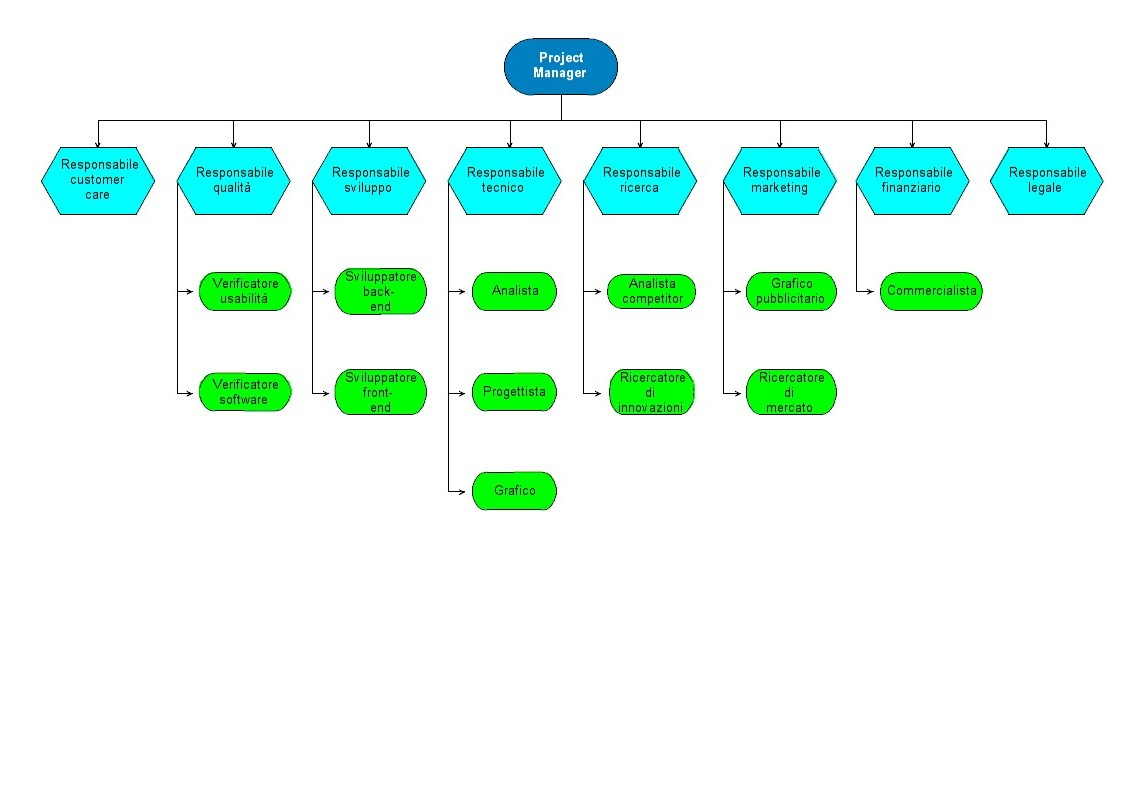
\includegraphics[scale=0.5]{img/Progetto2.jpg}
\caption{Diagramma OBS}
\label{fig:Diagramma OBS}
\end{figure}

\subsubsection{Project manager}
Responsabile ultimo del completamento del progetto, i suoi obblighi comprendono:
\begin{itemize}
\item realizzazione del progetto nel rispetto dei requisiti funzionali, di qualit\`{a} e dei
vincoli imposti;
\item rispetto dei tempi di consegna e dei costi preventivati;
\item rispetto dei margini di profitto preventivati.
Per assicurarsi di far fronte ai suoi obblighi, il PM pianifica tutte le fasi del progetto
coordinando le risorse per assicurare il conseguimento degli obbiettivi, anche in caso di
circostanze inaspettate.
\end{itemize}

\subsubsection{Responsabile costumer care}
Il RCC deve:
\begin{itemize}
\item scegliere le modalit\`{a} con cui gli utenti possono comunicare all\textquoteright{}azienda;
\item scegliere i servizi a cui appoggiarsi per gestire il rapporto con i clienti;
\item intrattenere rapporti diretti con i clienti pi\`{u} importanti, eventualmente con il
supporto del PM;
\item stendere rapporti mensili (da consegnare al PM) inerenti le maggiori problematiche
riscontrate dai clienti o con i mezzi di comunicazione e i servizi adottati.
\end{itemize}

\subsubsection{Responsabile qualit\`{a}}
Il RQ ha il compito di definire gli standard di qualit\`{a} da rispettare per ogni singolo processo
svolto dall\textquoteright{}azienda e di promuovere il miglioramento dei processi in corso di sviluppo.
Si attiene strettamente alle normative in materia di qualit\`{a} (ISO 9000/9001/9004
e ISO 9126 relativamente alla qualit\`{a} del software) e, a seguito dell\textquoteright{} analisi dei singoli
processi, promuove azioni di miglioramento, sia attraverso comunicazioni interne all\textquoteright{}azienda,
che attraverso formazione specifica degli addetti. Il miglioramento continuo
della qualit\`{a} aziendale, seguendo le linee guida del CMMI\footnote{Capability Maturity Model Integration - \url{http://it.wikipedia.org/wiki/Capability\_Maturity\_Model}}, garantisce all\textquoteright{}azienda un
miglioramento dell\textquoteright{}efficienza ed una maggiore soddisfazione dei clienti. Per quanto riguarda
il prodotto software sviluppato, il RQ deve inoltre comunicare al PM i verbali
ottenuti dai suoi sottoposti e proporre attivit\`{a} mirate all\textquoteright{}incremento della qualit\`{a}.

\subsubsection{Verificatore usabilit\`{a}}
L\textquoteright{}azienda crede fermamente che un prodotto altamente usabile (vedi ISO 9241) sia
sinonimo di qualit\`{a} e sia in parte garanzia di successo. Per questo motivo, contemporaneamente
alla verifica di accessibilit\`{a} del prodotto, il verificatore valuter\`{a} eventuali
migliorie sul piano dell\textquoteright{}usabilit\`{a} e rediger\`{a} un verbale per il RQ esponendo le eventuali problematiche riscontrate e le possibili soluzioni.

\subsubsection{Verificatore software}
Tra le varie fasi che compongono la creazione di un prodotto software, c\textquoteright{}\`{e} il testing.
Questa operazione viene svolta dagli sviluppatori (SF e SB) e punta all\textquoteright{}eliminazione del
maggior numero di bug possibili. Una fase altrettanto importante \`{e} quella della verifica
e della validazione del software (vedi IEEE 1012), in questo caso il VS deve controllare
che quanto prodotto rispetti i requisiti espressi nel documento di Analisi dei Requisiti
redatto dall\textquoteright{}analista e sia effettivamente quanto richiesto. Al termine di ogni sessione di verifica il VS rediger\`{a} un verbale per il RQ.

\subsubsection{Responsabile tecnico}
Il RT coordina ogni fase dello sviluppo dei prodotti software dell\textquoteright{}azienda ed \`{e} il responsabile
dello stato di avanzamento dei prodotti nel rispetto delle scadenze temporali e
dei costi. Ha una competenza tecnica molto vasta e deve potersi
relazionare con i suoi subordinati su ogni aspetto dello sviluppo.\\
Una volta ricevuto l\textquoteright{}incarico dal PM:
\begin{enumerate}
\item assegna all\textquoteright{}analista il compito di formalizzare quanto dev\textquoteright{}essere prodotto;
\item al termine della fase di analisi, incarica:
\begin{itemize}
\item il Progettista di delineare l\textquoteright{}architettura di dettaglio;
\item il Grafico di stendere le bozze delle interfacce utente.
\end{itemize}
\item durante la fase di progettazione, il RT controlla che l\textquoteright{}architettura software rispetti
le metriche software concordate e propone al progettista eventuali modifiche. Nel
caso fosse necessario (utilizzo di un nuovo linguaggio/framework), predispone corsi
di aggiornamento o di formazione per gli sviluppatori;
\item al termine della fase di progettazione, consegna quanto prodotto al RS;
\item coordina le operazioni di manutenzione successive al rilascio.
\end{enumerate}

\subsubsection{Analista}
L\textquoteright{}analista ha il compito di formalizzare quanto emerso dalle discussioni con il PM e
dalla lettura della documentazione di presentazione del progetto. Redige lo "Studio di Fattibilit\`{a}", nel quale si indica se il progetto \`{e} fattibile e quali sono le aree critiche ed il documento di Analisi dei Requisiti nel quale, con l\textquoteright{}ausilio di diagrammi dei casi d\textquoteright{}uso e di altri formalismi(vedi INCOSE\footnote{International Council on Systems Engineering - \url{http://www.incose.org/}}), viene riportato cosa sar\`{a} sviluppato. Al termine della fase di analisi l\textquoteright{}analista consegner\`{a} entrambi i documenti al RT.

\subsubsection{Progettista}
La fase di progettazione ha inizio con la delibera, da parte del PM, di quanto prodotto
dall\textquoteright{}analista e con la conseguente assegnazione dell\textquoteright{}incarico al Progettista. Una volta
studiata l\textquoteright{}Analisi dei Requisiti, il progettista redige dapprima il documento di "Specifica
Tecnica", nel quale viene proposta una soluzione ad alto livello del problema focalizzandosi
maggiormente sulle funzionalit\`{a}, piuttosto che sulla loro implementazione, e successivamente
il documento di "Definizione di Prodotto" nel quale si propone una soluzione concreta e
dettagliata al problema posto. In entrambi i documenti il progettista far\`{a} ampio uso di
diagrammi e schemi per rendere il pi\`{u} chiara possibile qualsiasi scelta implementativa.
Al termine della fasi di progettazione i documenti prodotti sono consegnati al RT.

\subsubsection{Grafico}
Il grafico viene incaricato dal RT di creare le bozze per ogni interfaccia utente presente
nel progetto. Il lavoro inizia con la lettura dell\textquoteright{}"Analisi dei Requisiti" e, in particolare,
con la sezione relativa ai casi d\textquoteright{}uso che indicano, tra l\textquoteright{}altro, quante possibili bozze sono
necessarie. Una volta create, le bozze vengono consegnate al PM che le valuta con
l\textquoteright{}ausilio del team del RQ e, se necessario, con il RDM.

\subsubsection{Responsabile sviluppo}
Il RS coordina ogni fase dello sviluppo dei prodotti software dell\textquoteright{}azienda ed \`{e} il responsabile
dello stato di avanzamento dei prodotti nel rispetto delle scadenze temporali e
dei costi. Ha una competenza tecnica molto vasta assimilata e deve potersi
relazionare con i suoi subordinati su ogni aspetto dello sviluppo. Una volta ricevuto
l\textquoteright{}incarico dal RT in accordo con il PM:
\begin{itemize}
\item suddivide gli incarichi di lavoro tra SF e SB in base a quanto fornito dal RT;
\item durante la fasi di sviluppo, segue attentamente i report relativi ai test effettuati e
controlla lo stato di avanzamento del prodotto in relazione alle scadenze prefissate;
\item supervisiona le fasi di alpha e beta testing ed i successivi test di collaudo precedenti
il rilascio.
\end{itemize}

\subsubsection{Sviluppatore front-end}
Lo SF viene incaricato dal RS di realizzare e successivamente manutenere tutte le parti
software con cui interagisce l\textquoteright{}utente, oltre ai documenti tecnici prodotti dal Progettista
gli vengono consegnate anche le bozze create dal Grafico.

\subsubsection{Sviluppatore back-end}
Lo SB viene incaricato dal RS di realizzare e successivamente manutenere tutte le parti
software che elaborano dati e non sono a diretto contatto con l\textquoteright{}utente, per svolgere il
suo compito necessita solo dei documenti tecnici prodotti dal Progettista.

\subsubsection{Responsabile ricerca}
Il mercato attuale \`{e} in continua evoluzione ed anche potendo contare su un prodotto
di successo, bisogna essere in grado di migliorarlo continuamente per poter rimanere al
passo rispetto alla concorrenza. Il RR quindi coordina il suo team per:
\begin{itemize}
\item rimanere al passo con i competitor, analizzando le funzionalit\`{a} da loro
implementate e capendo quali di esse potrebbero dare un valore aggiunto al
progetto;
\item creare un gap rispetto ai competitor, cercando soluzioni innovative non ancora
presenti sul mercato e che facciano evolvere positivamente il progetto.
\end{itemize}

\subsubsection{Analista competitor}
L\textquoteright{}AC deve scandagliare tutti i "rivali" del prodotto che si sta sviluppando e cercare
di capire quali delle soluzioni da loro implementate possano dare un tangibile valore
aggiunto al progetto. A ricerca completata l\textquoteright{}AC produrr\`{a} una documentazione di quanto
trovato e la consegner\`{a} per valutazione al RR.

\subsubsection{Ricercatore di innovazioni}
Il RI basandosi su quanto reso disponibile dal prodotto e su eventuali trend di mercato
in settori affini, cerca di trovare novit\`{a} da poter implementare nel prodotto al fine di
aumentare: le funzionalit\`{a} offerte, la soddisfazione dell\textquoteright{}utente, il bacino di utenza e di
estendere eventualmente il target del prodotto. Al termine del processo il RI produrr\`{a}
una documentazione che sar\`{a} consegnata per valutazione al RR.

\subsubsection{Responsabile marketing}
Il RM ha l\textquoteright{}onere di posizionare i prodotti nel mercato di riferimento e di renderli profittevoli.
Per adempiere al suo compito analizza il mercato individuando cos\`{i} le opportunit\`{a}
di business e progetta ed attua le strategie di marketing pi\`{u} efficaci per l\textquoteright{}incremento
dei profitti e per l\textquoteright{}affermazione del brand.

\subsubsection{Grafico Pubblicitario}
Per far conoscere l\textquoteright{}azienda ai possibili utilizzatori e per stimolare l\textquoteright{}adozione dei prodotti
proposti \`{e} indispensabile avere campagne pubblicitarie efficaci. Il GP, sotto la
supervisione del RM, crea le pubblicit\`{a} dell\textquoteright{}azienda.

\subsubsection{Ricercatore di mercato}
Il RDM ha competenze statistiche specifiche nella creazione di sondaggi e nell\textquoteright{}analisi
dei dati ottenuti; ha lo scopo di comprendere qual \`{e} l\textquoteright{}opinione delle persone relativamente
all\textquoteright{}azienda e ai prodotti da essa sviluppati e quali sono, in generale, gli aspetti
migliorabili. Si occupa, quindi, di redigere sondaggi ai fini di comprendere:
\begin{itemize}
\item qual \`{e} il target di riferimento;
\item quanto gli utenti conoscono i prodotti sviluppati dall\textquoteright{}azienda;
\item il livello di qualit\`{a} e seriet\`{a} che gli utenti attribuiscono all\textquoteright{}azienda e ai suoi
prodotti;
\item eventuali aspetti negativi riscontrati o miglioramenti proposti.
\end{itemize}

\subsubsection{Responsabile finanziario}
Il RF ha il compito di monitorare il flusso di cassa dell\textquoteright{}azienda e di individuare eventuali
problematiche ben prima che si verifichino. Si avvale di un Commercialista per le
operazioni contabili e di un BF per massimizzare le rendite dell\textquoteright{}azienda.

\subsubsection{Commercialista}
Il Commercialista \`{e} incaricato dall\textquoteright{}azienda di mantenerne la contabilit\`{a}, di effettuare i
versamenti delle tasse e di verificare e legittimarne le operazioni economiche.

\subsubsection{Responsabile legale}
Il RL viene contattato dall\textquoteright{}azienda quando:
\begin{itemize}
\item si vuole garantire che i software sviluppati rispettino le normative vigenti, nello
specifico quelle relative alla privacy;
\item si vogliono archiviare particolari brevetti o si vuole garantire il copyright di un
prodotto;
\item nascono dispute legali tra terzi e l\textquoteright{}azienda;
\item si sviluppano trattative economiche delle quali non \`{e} del tutto chiara la legittimit\`{a}.
\end{itemize}


\subsection{Resource Breakdown Structure}
La Resource Breakdown Structure, d'ora in poi RBS, identifica ed esplicita tutte le
risorse necessarie alla realizzazione del progetto. Queste vengono classificate a seconda della
loro categoria e tipologia. Con il termine risorsa si intende specificare ogni singola
componente fra tutto quello che risulta essere utile e necessario per lo svolgimento e la
buona riuscita del progetto: le risorse umane, i materiali, le attrezzature ed il tempo;
ovvero componenti a cui sia possibile attribuire un costo in denaro per il loro utilizzo. La
RBS si dimostra un ottimo strumento di supporto alla pianificazione in quanto consente
di ottimizzare l'impiego di ogni singola risorsa necessaria, inoltre la RBS risulta essere fortemente
legata alla stima dei costi in quanto questi vengono generati in base all'impiego delle
risorse descritte.

\begin{figure}[H]
\centering % per centrare l'immagine (opzionale)
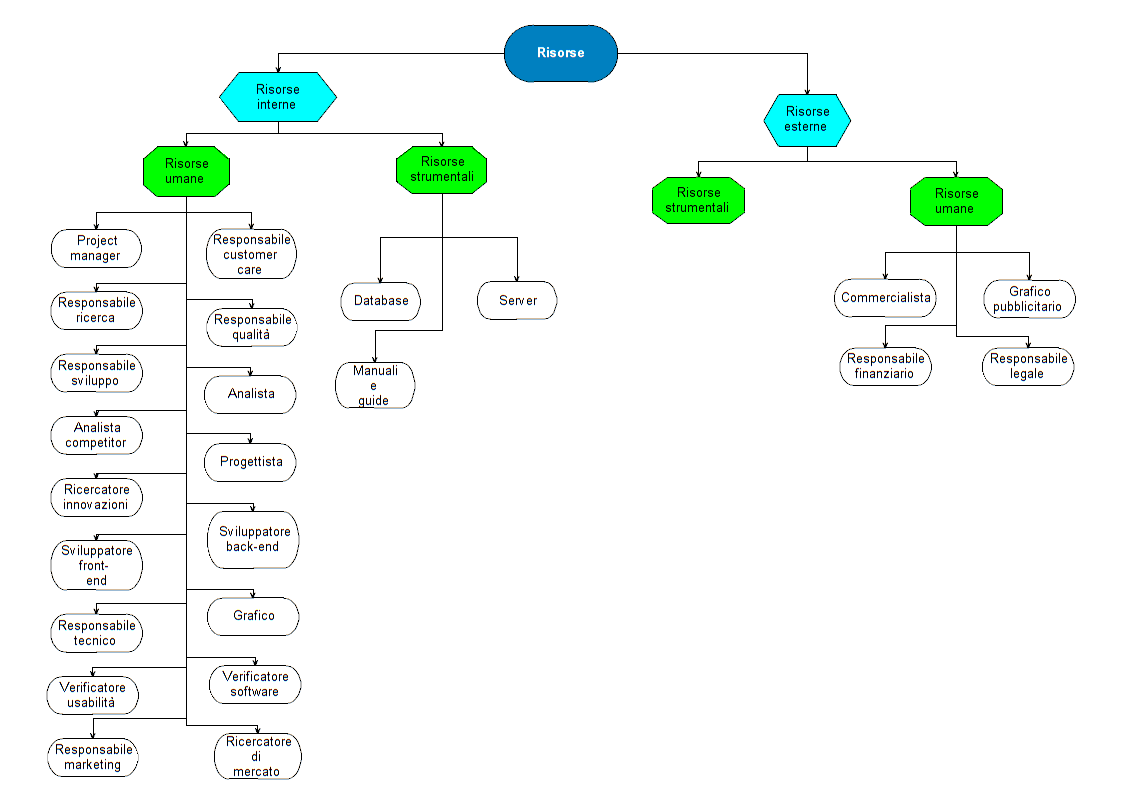
\includegraphics[scale=0.5]{img/Risorse_rbs.png}
\caption{Diagramma RBS}
\label{fig:Diagramma RBS}
\end{figure}


\subsection{Pianificazione temporale}
\subsubsection{Diagramma di Gantt}

I diagrammi di Gantt sono una rappresentazione su scala temporale dell'evoluzione del
progetto. Sono composti da varie barre orizzontali ognuna delle quali rappresenta una
attivit\'a che viene collocata sulla scala temporale in rappresentanza dell'attivi\'a stessa.
I diagrammi di Gantt hanno lo scopo di:
\begin{itemize}
\item definire cosa fare in una certa quantit\'a di tempo;
\item definire un riferimento per il controllo dell'avanzamento;
\item  definire degli eventi chiave dette milestones (fine di una fase, consegna).
\end{itemize}
Un diagramma di Gantt consente quindi la rappresentazione grafica di un calendario di
attivit\'a facilitando la pianificazione, il coordinamento e il tracciamento delle specifiche
attivit\'a dando una illustrazione dello stato di avanzamento del progetto. Per costruire
un diagramma di Gantt bisogna:
\begin{itemize}
\item  determinare le attivit\'a necessarie per concludere il progetto;
\item  stabilire il limite temporale del progetto;
\item  disegnare sul grafico il limite temporale stimato per ciascuna attivit\'a;
\item  verificare la presenza di discrepanze tra il tempo stimato e quello effettivamente
utilizzato.
\end{itemize}
Tramite i diagrammi di Gantt si identifica il percorso critico: alcune attivit\'a possono
partire solo dopo che altre sono finite, ognuna di queste attivit\'a viene detta critica e la
loro unione forma il percorso critico. \'E molto importante che le attivit\'a critiche non
subiscano slittamenti poich\'e questi si ripercuoterebbero, a cascata, su tutte le attivit\'a
critiche in attesa.

\subsubsection{Microsoft Project 2013}
Per la gestione e la pianificazione del progetto si \'e scelto di usare Project2013 essendo
un software dedicato al Project Management. Project2013 
crea automaticamente i diagrammi di Gantt una volta inserite le singole attivit\'a. Il software permette, inoltre, di modificare
le relazioni tra le attivit\'a e le date di inizio e fine nel caso le previsioni fatte non si
verifichino veritiere, o per l'insorgenza di problemi inaspettati. Questa funzionalit\'a
permette di mantenere il piano di progetto aggiornato con gli ultimi avvenimenti e d\'a
un idea del ritardo (o anticipo) acquisiti.

\subsubsection{Visione Globale del Progetto}
Viene presentata in questa sezione la visione generale del piano di progetto in modo da
dare una visione delle dipendenze tra le varie fasi, consentendo di comprendere:
\begin{itemize}
\item l'evoluzione temporale dell'intero progetto;
\item quanto pesa percentualmente ogni fase sia in senso economico che di tempo;
\item l'impiego delle varie risorse.
\end{itemize}
Di seguito sono presentate le immagini dei work package, ossia delle macro-attivit\'a in cui
\'e stato suddiviso il progetto, il diagramma di Gantt dell'intero progetto.
Il progetto risulta quindi avere un costo di \euro{}, a cui si dovranno andare a
sommare i costi di mantenimento e hosting del servizio.

\begin{figure}[H]
\begin{center}
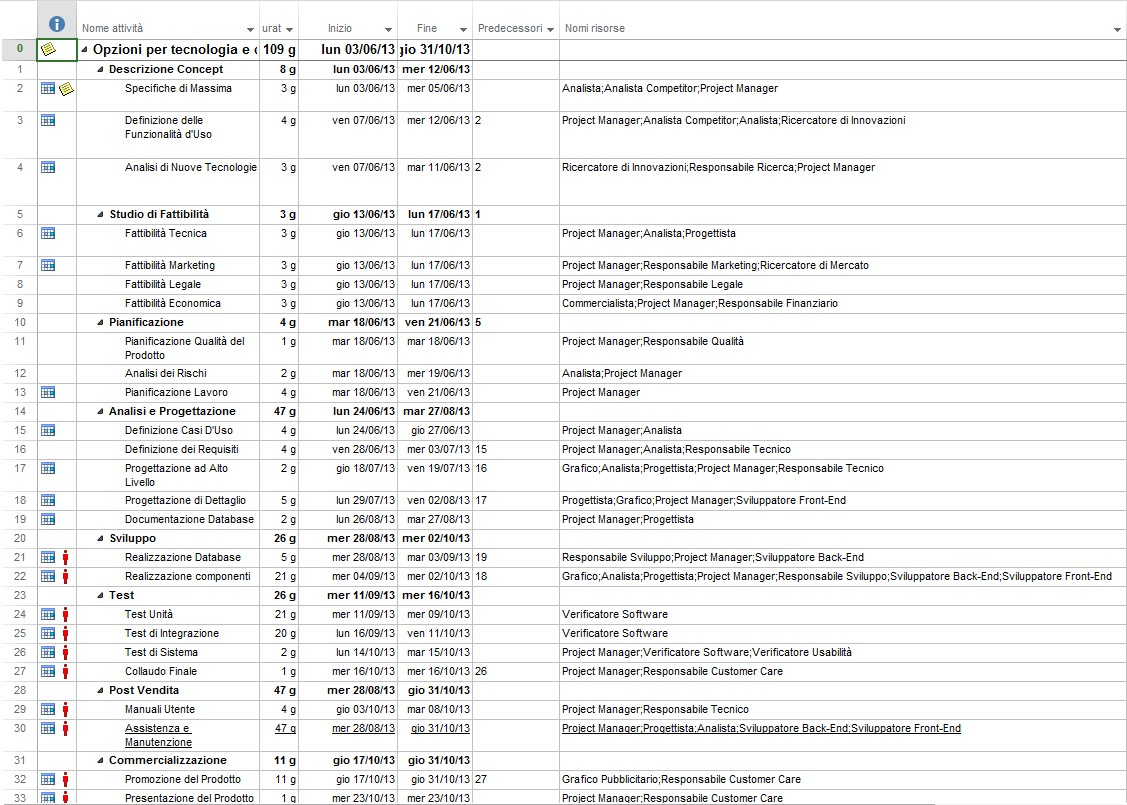
\includegraphics[width=1\textwidth]{img/Attivita.jpg}
\caption{Diagramma  Attivit\'a}
\label{fig:Diagramma Attivit\'a}
\end{center}
\end{figure}
\begin{figure}[H]
\begin{center}
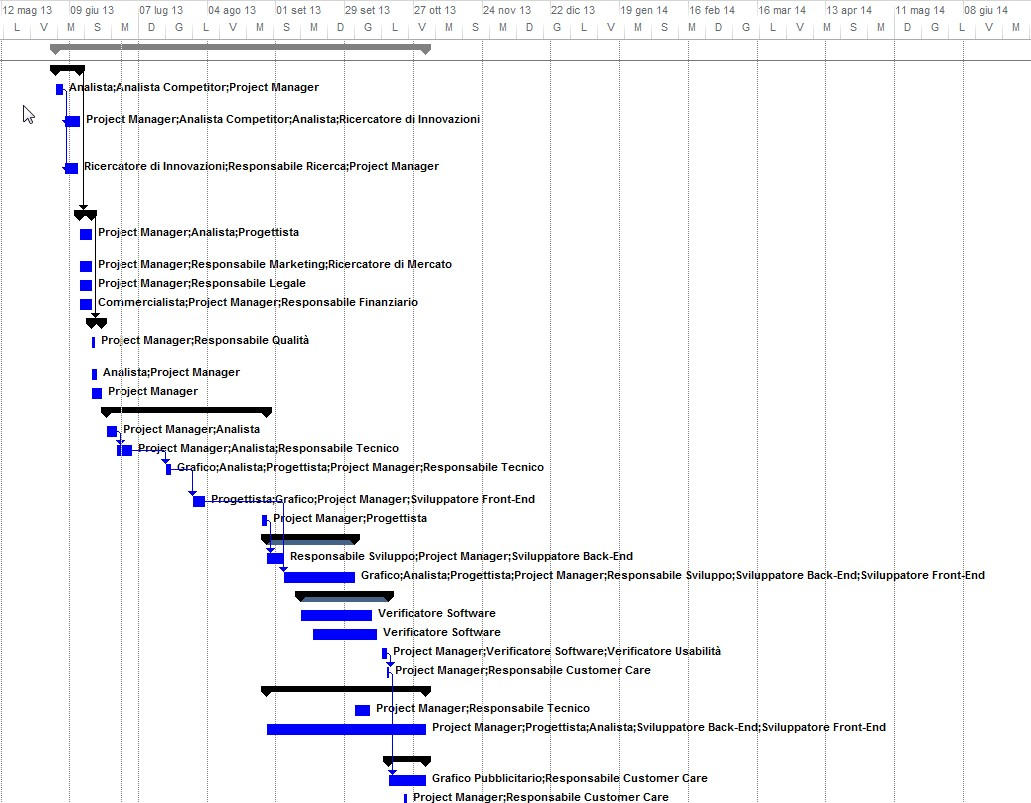
\includegraphics[width=1\textwidth]{img/Gantt.jpg}
\caption{Gantt Progetto}
\label{fig:Gantt Progetto}
\end{center}
\end{figure}
\newpage
\subsubsection{Gantt Milestone}

\begin{figure}[H]
\begin{center}
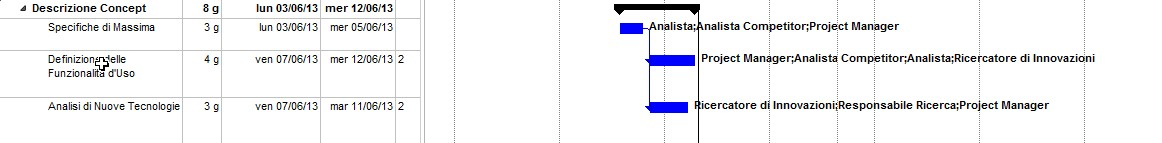
\includegraphics[width=1\textwidth]{img/G-A Concept.jpg}
\caption{Gantt Definizione Concept}
\label{fig:Gantt Definizione Concept}
\end{center}
\end{figure}

\begin{figure}[H]
\begin{center}
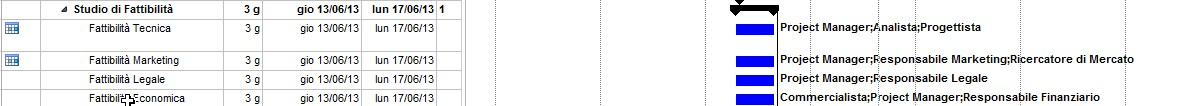
\includegraphics[width=1\textwidth]{img/G-A Fattibilita.jpg}
\caption{Gantt Studio di Fattibilit\'a}
\label{fig:Gantt Studio di Fattibilit\'a}
\end{center}
\end{figure}

\begin{figure}[H]
\begin{center}
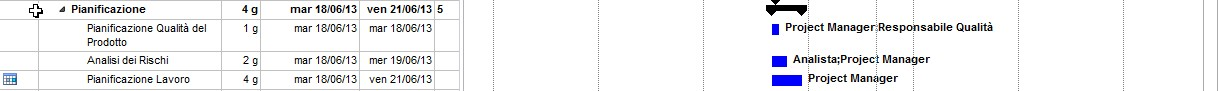
\includegraphics[width=1\textwidth]{img/G-A Pianificazione.jpg}
\caption{Gantt Pianificazione}
\label{fig:Gantt Pianificazione}
\end{center}
\end{figure}

\begin{figure}[H]
\begin{center}
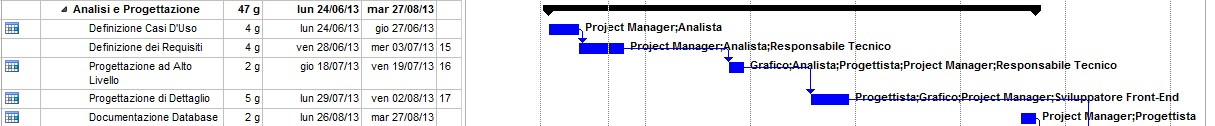
\includegraphics[width=1\textwidth]{img/G-A Analisi.jpg}
\caption{Gantt Analisi e Progettazione}
\label{fig:Gantt Analisi e Progettazione}
\end{center}
\end{figure}

\begin{figure}[H]
\begin{center}
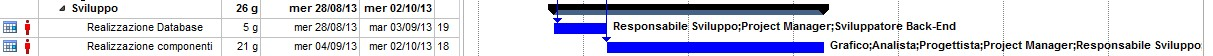
\includegraphics[width=1\textwidth]{img/G-A Sviluppo.jpg}
\caption{Gantt Sviluppo}
\label{fig:Gantt Sviluppo}
\end{center}
\end{figure}

\begin{figure}[H]
\begin{center}
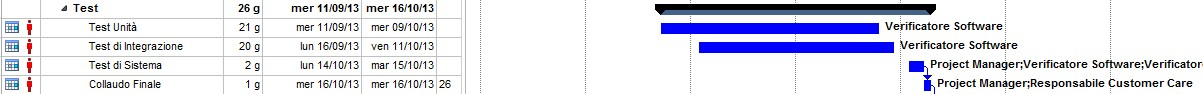
\includegraphics[width=1\textwidth]{img/G-A Test.jpg}
\caption{Gantt Test}
\label{fig:Gantt Test}
\end{center}
\end{figure}

\begin{figure}[H]
\begin{center}
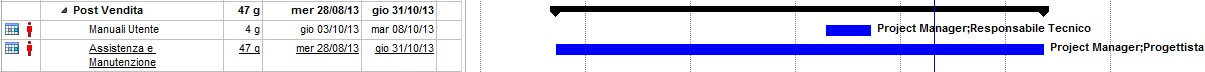
\includegraphics[width=1\textwidth]{img/G-A Vendita.jpg}
\caption{Gantt Vendita}
\label{fig:Gantt Vendita}
\end{center}
\end{figure}

\begin{figure}[H]
\begin{center}
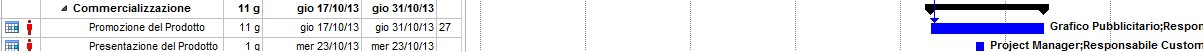
\includegraphics[width=1\textwidth]{img/G-A Commercializzazione.jpg}
\caption{Gantt Commercializzazione}
\label{fig:Gantt Commercializzazione}
\end{center}
\end{figure}